\subsection{iPerceive: Applying Common-Sense Reasoning to Multi-Modal Dense Video Captioning and Video Question Answering}

\subsubsection{Overview}

\par Aman Chadha \textit{et al}, in their 2017 paper titled \textit{iPerceive: Applying Common-Sense Reasoning to Multi-Modal Dense Video Captioning and Video Question Answering} \cite{chadha2020iperceive}, proposed to understand the \textit{"why"} between the events \textit{P(Y | do(X))} by handling
\textit{cognitive error} (giving importance to past events which leads to future events) and \textit{incorrect attention} (attending to every major object in the frame (eg. recognizing oven from the cooking video)). They used video frames, audio and speech text in end-to-end manner for inference.


\subsubsection{Datasets}
\begin{itemize}
\item ActivityNet Captions
\item TVQA (for video question answering task)
\end{itemize}

\subsubsection{Performance}
\par Chadha \textit{et al} compared captioning results with Krishna \textit{et al}\cite{krishna2017densecaptioning}, Wang \textit{et al}\cite{wang2018bidirectional}, Zhou \textit{et al}\cite{zhou2018end}, Li \textit{et al}\cite{li2018jointly}, Iashin \textit{et al}\cite{iashin2020multimodal} and Rahman \textit{et al}\cite{rahman2019watch} using BLEU@3-4 and METEOR. The model performed better with both ground-truth and learnt proposals. They also benchmark the modified model on task of video question answering. 


\subsubsection{Methodology}

\par Chadha \textit{et al} architecture consists of three main components:
\begin{enumerate}
	\item Event proposal module
	\item Common-sense reasoning module
	\item Captioning module
\end{enumerate}

\begin{figure}[h]
	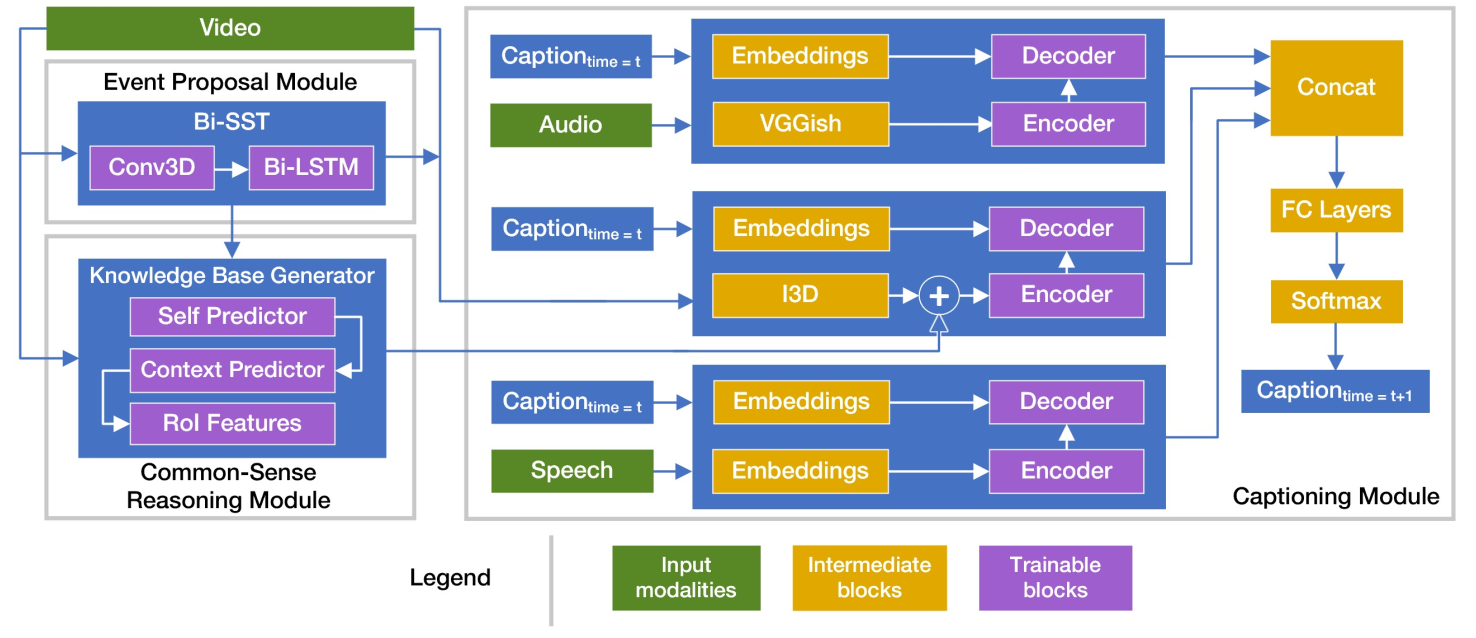
\includegraphics[width=\linewidth]{assets/img/chadha2020iperceive-architecture.png}
	\caption{Architecture introduced by Chadha \textit{et al} (Image courtesy \cite{chadha2020iperceive})}
\end{figure}

\paragraph{Event Proposal Module} - Temporally localize a set of events in a video
\begin{enumerate}
	\item Bidirectional Single Stream Network (Bi-SST)\cite{wang2018bidirectional} for localizing events.
	\item Bi-SST applies 3D convolutions to video frames and passes on the extracted features to a Bi-directional LSTM network.
	\item Output is the endpoints of each event along with its confidence score.
\end{enumerate}

\paragraph{Common-Sense Reasoning Module} - Build a knowledge base for common sense reasoning
\begin{enumerate}
	\item This module generates visual features for the events detected.
	\item Determines causality: P(Y | do(X)) using borrow-put experiment.
	\item The features generated by this module are then paired with corresponding visual features and sent to captioning module.
\end{enumerate}

\paragraph{Captioning Module} - Produce textual description using audio, video and speech cues for each event
\begin{enumerate}
	\item Given an event proposal and its common-sense vectors, the captioning module generates a caption using audio, visual and speech modalities.
	\item Transformer-based architecture.
	\item Omits the self-multi-head attention component since it applies P(Y | X) rather than the main motive P(Y | do(X)).
\end{enumerate}


\subsubsection{Conclusion}

\par Chadha \textit{et al} introduced the concept of common-sense features in dense video captioning. Furthermore, the end-to-end architecture helps in learning relationship between events and language. 